% Appendix figures for results.tex. In report/midway/main.tex, after \appendix:
%   \section{Additional results}
%   % Appendix figures for results.tex. In report/midway/main.tex, after \appendix:
%   \section{Additional results}
%   % Appendix figures for results.tex. In report/midway/main.tex, after \appendix:
%   \section{Additional results}
%   % Appendix figures for results.tex. In report/midway/main.tex, after \appendix:
%   \section{Additional results}
%   \input{results_appendix}
% Figure paths are set by \graphicspath in results.tex.

\begin{figure}[!h]
  \centering
  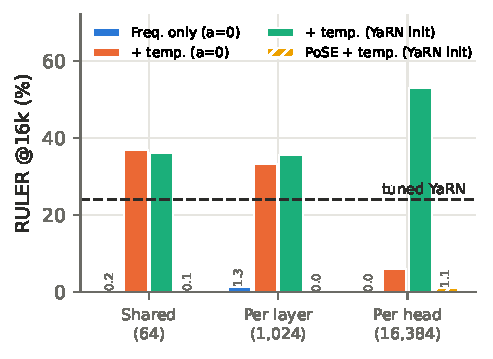
\includegraphics[width=\columnwidth]{fig_ablation_16k.pdf}
  \caption{RULER at 16k per granularity. Blue vs.\ orange differ only in the
  learned temperature; green starts both at YaRN; hatched yellow is PoSE
  (trained on 4k text). Dashed: tuned YaRN.}
  \label{fig:ablation}
\end{figure}

\begin{figure}[!h]
  \centering
  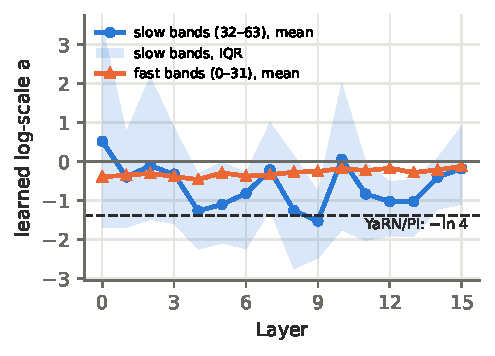
\includegraphics[width=\columnwidth]{fig_learned_a.pdf}
  \caption{Learned log frequency scales $a$ of the per-layer, frequencies-only
  model ($a<0$: slower rotation, $a=0$: unchanged). Line: mean over bands;
  shaded: middle 50\% of slow bands. Dashed: the single value YaRN and PI use
  for slow bands.}
  \label{fig:learned-a}
\end{figure}

\begin{figure}[!h]
  \centering
  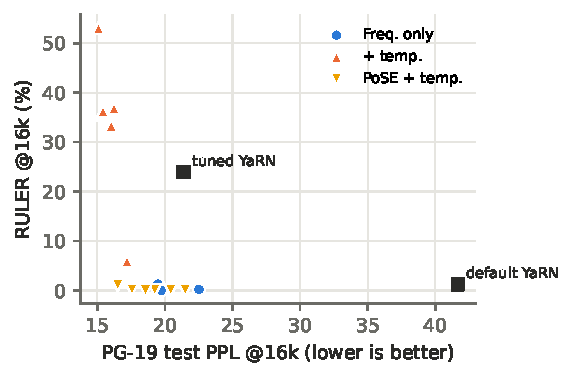
\includegraphics[width=\columnwidth]{fig_ppl_vs_ruler.pdf}
  \caption{Perplexity and retrieval at 16k disagree. Each marker is one trained
  model. Frequencies-only models (blue) and PoSE models (yellow) have perplexity
  similar to or better than tuned YaRN but almost no retrieval.
  The original model and PI are off the scale and not shown.}
  \label{fig:ppl-ruler}
\end{figure}

\begin{figure*}[!t]
  \centering
  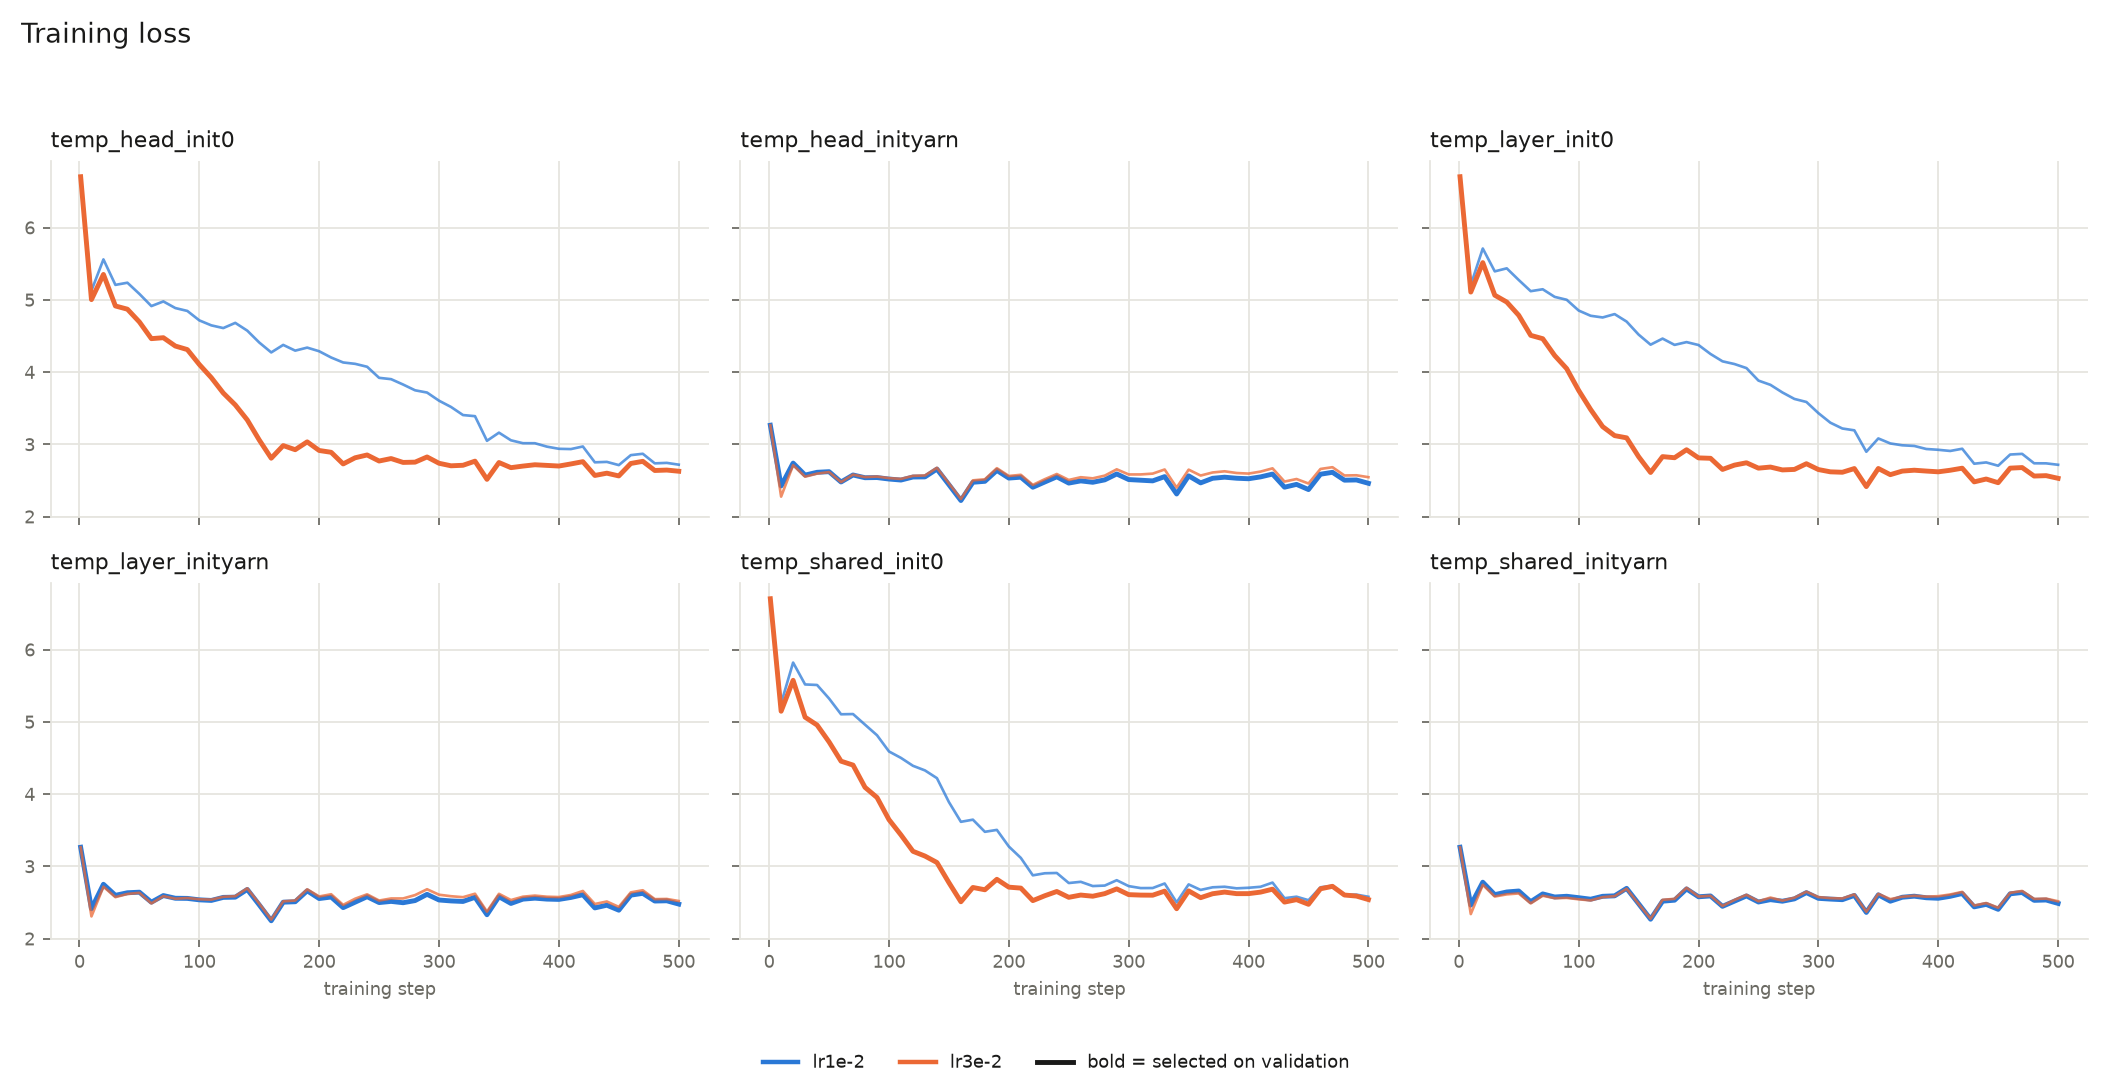
\includegraphics[width=\textwidth]{loss.png}
  \caption{Training loss of the frequencies + temperature runs for each
  granularity and starting point, at two learning rates (bold: chosen on
  validation). Runs started at YaRN begin near their final loss; runs from
  $a{=}0$ need hundreds of steps.}
  \label{fig:loss}
\end{figure*}

% Figure paths are set by \graphicspath in results.tex.

\begin{figure}[!h]
  \centering
  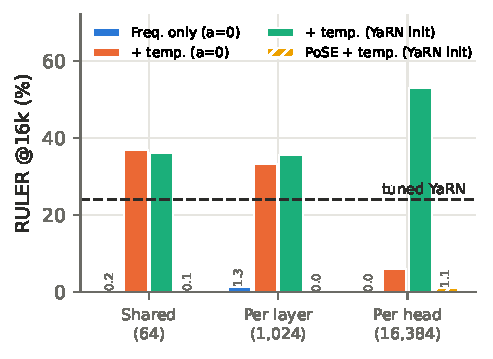
\includegraphics[width=\columnwidth]{fig_ablation_16k.pdf}
  \caption{RULER at 16k per granularity. Blue vs.\ orange differ only in the
  learned temperature; green starts both at YaRN; hatched yellow is PoSE
  (trained on 4k text). Dashed: tuned YaRN.}
  \label{fig:ablation}
\end{figure}

\begin{figure}[!h]
  \centering
  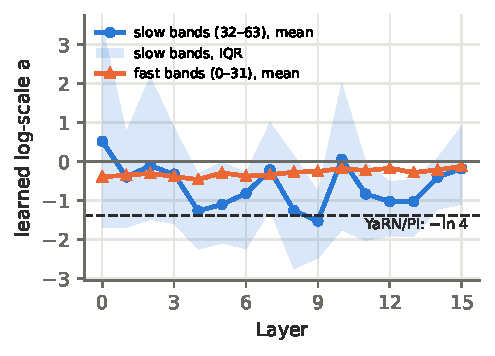
\includegraphics[width=\columnwidth]{fig_learned_a.pdf}
  \caption{Learned log frequency scales $a$ of the per-layer, frequencies-only
  model ($a<0$: slower rotation, $a=0$: unchanged). Line: mean over bands;
  shaded: middle 50\% of slow bands. Dashed: the single value YaRN and PI use
  for slow bands.}
  \label{fig:learned-a}
\end{figure}

\begin{figure}[!h]
  \centering
  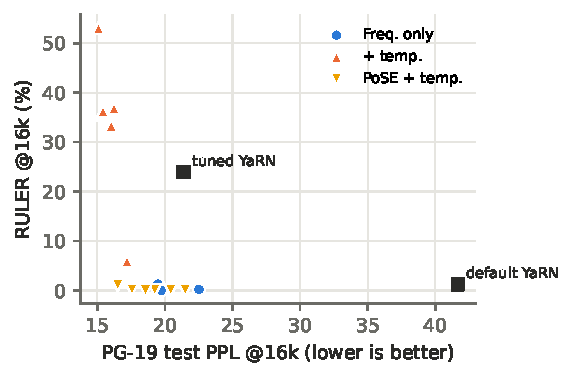
\includegraphics[width=\columnwidth]{fig_ppl_vs_ruler.pdf}
  \caption{Perplexity and retrieval at 16k disagree. Each marker is one trained
  model. Frequencies-only models (blue) and PoSE models (yellow) have perplexity
  similar to or better than tuned YaRN but almost no retrieval.
  The original model and PI are off the scale and not shown.}
  \label{fig:ppl-ruler}
\end{figure}

\begin{figure*}[!t]
  \centering
  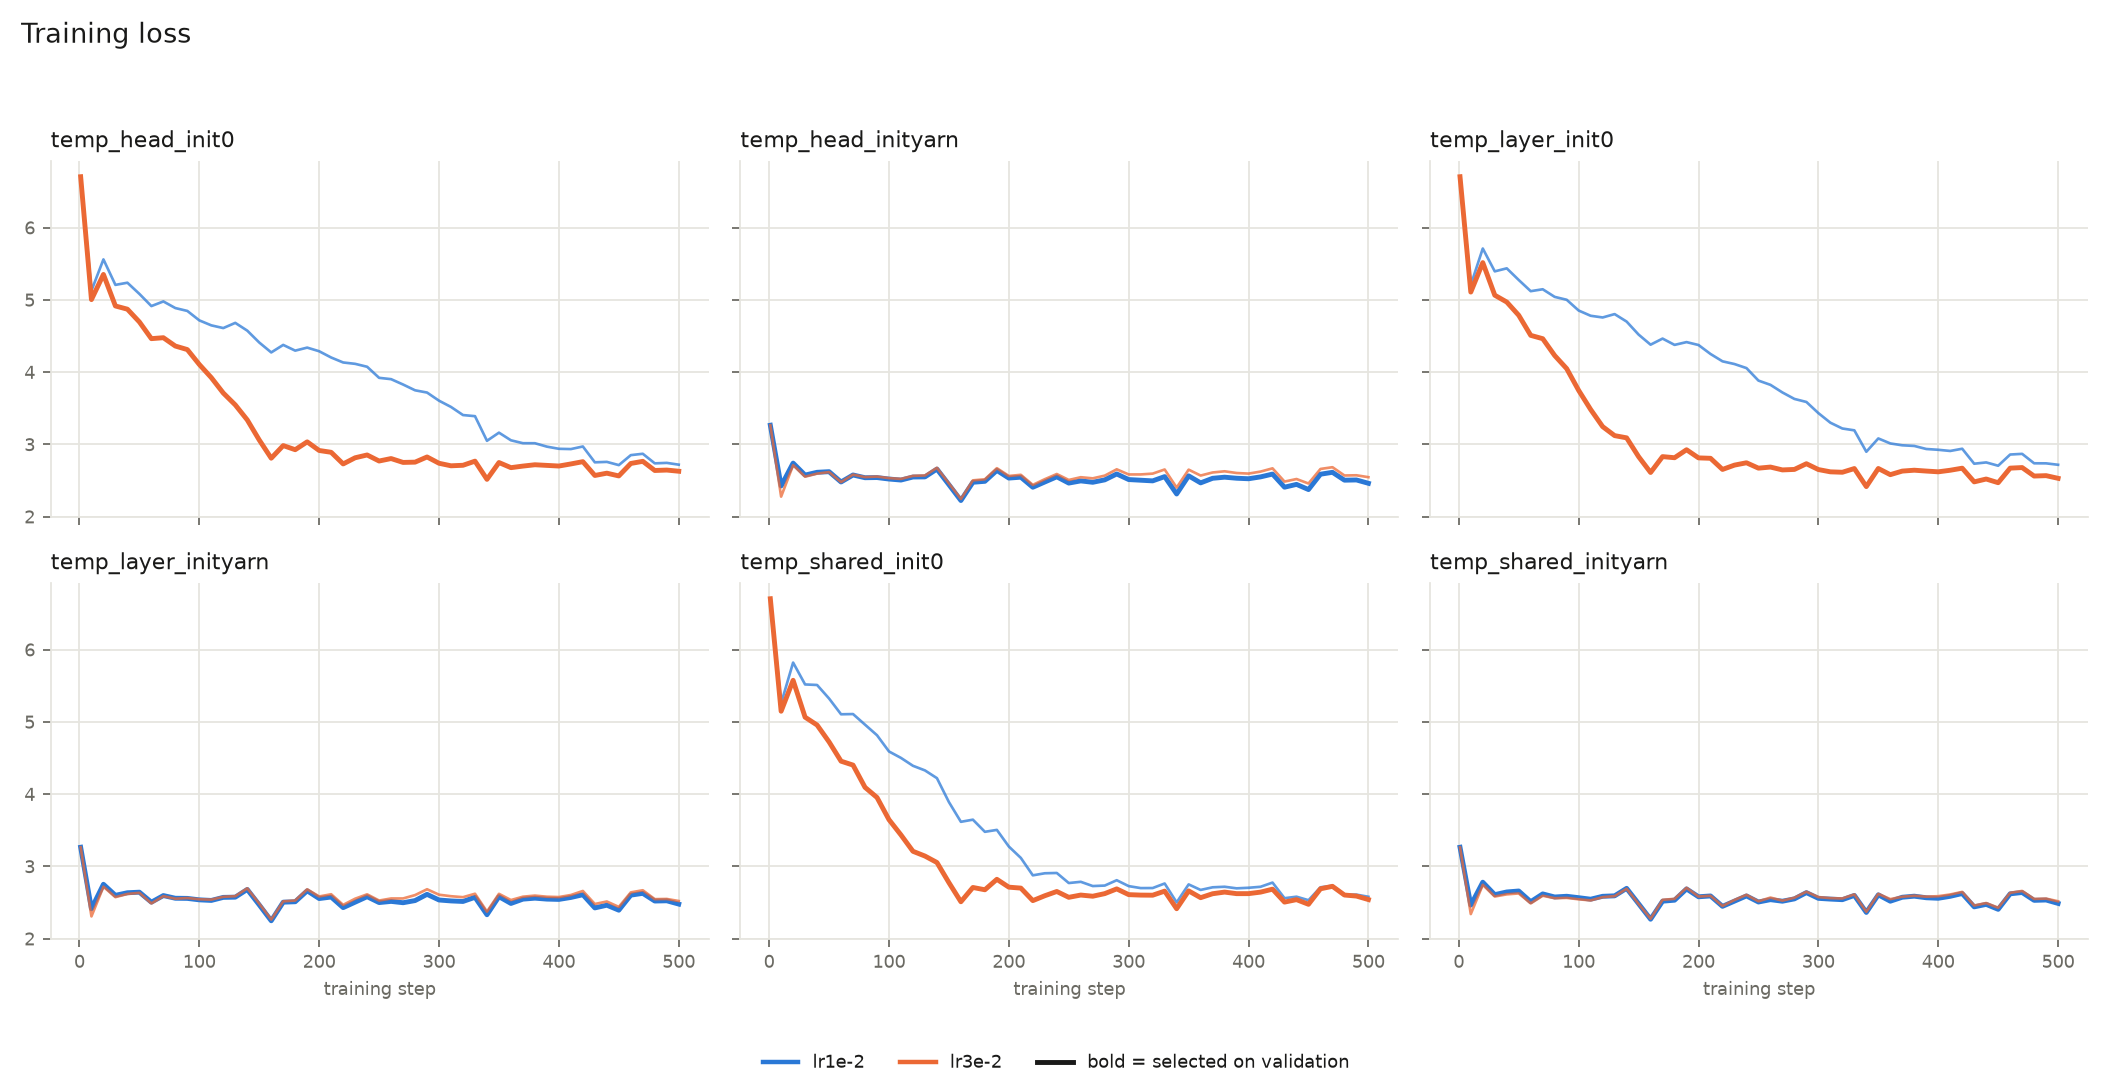
\includegraphics[width=\textwidth]{loss.png}
  \caption{Training loss of the frequencies + temperature runs for each
  granularity and starting point, at two learning rates (bold: chosen on
  validation). Runs started at YaRN begin near their final loss; runs from
  $a{=}0$ need hundreds of steps.}
  \label{fig:loss}
\end{figure*}

% Figure paths are set by \graphicspath in results.tex.

\begin{figure}[!h]
  \centering
  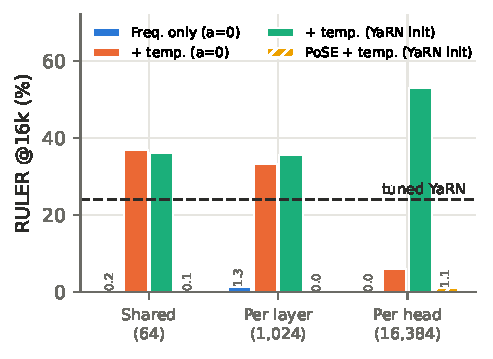
\includegraphics[width=\columnwidth]{fig_ablation_16k.pdf}
  \caption{RULER at 16k per granularity. Blue vs.\ orange differ only in the
  learned temperature; green starts both at YaRN; hatched yellow is PoSE
  (trained on 4k text). Dashed: tuned YaRN.}
  \label{fig:ablation}
\end{figure}

\begin{figure}[!h]
  \centering
  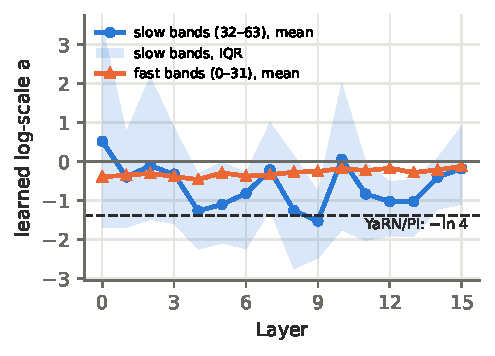
\includegraphics[width=\columnwidth]{fig_learned_a.pdf}
  \caption{Learned log frequency scales $a$ of the per-layer, frequencies-only
  model ($a<0$: slower rotation, $a=0$: unchanged). Line: mean over bands;
  shaded: middle 50\% of slow bands. Dashed: the single value YaRN and PI use
  for slow bands.}
  \label{fig:learned-a}
\end{figure}

\begin{figure}[!h]
  \centering
  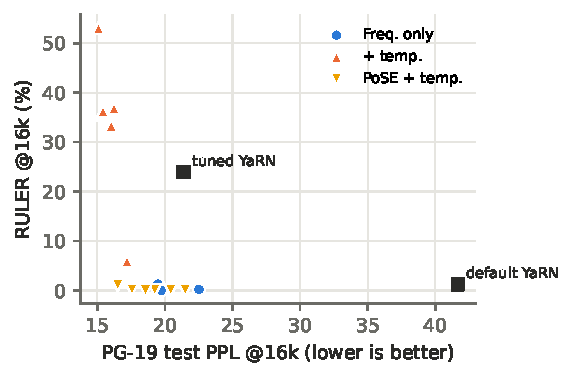
\includegraphics[width=\columnwidth]{fig_ppl_vs_ruler.pdf}
  \caption{Perplexity and retrieval at 16k disagree. Each marker is one trained
  model. Frequencies-only models (blue) and PoSE models (yellow) have perplexity
  similar to or better than tuned YaRN but almost no retrieval.
  The original model and PI are off the scale and not shown.}
  \label{fig:ppl-ruler}
\end{figure}

\begin{figure*}[!t]
  \centering
  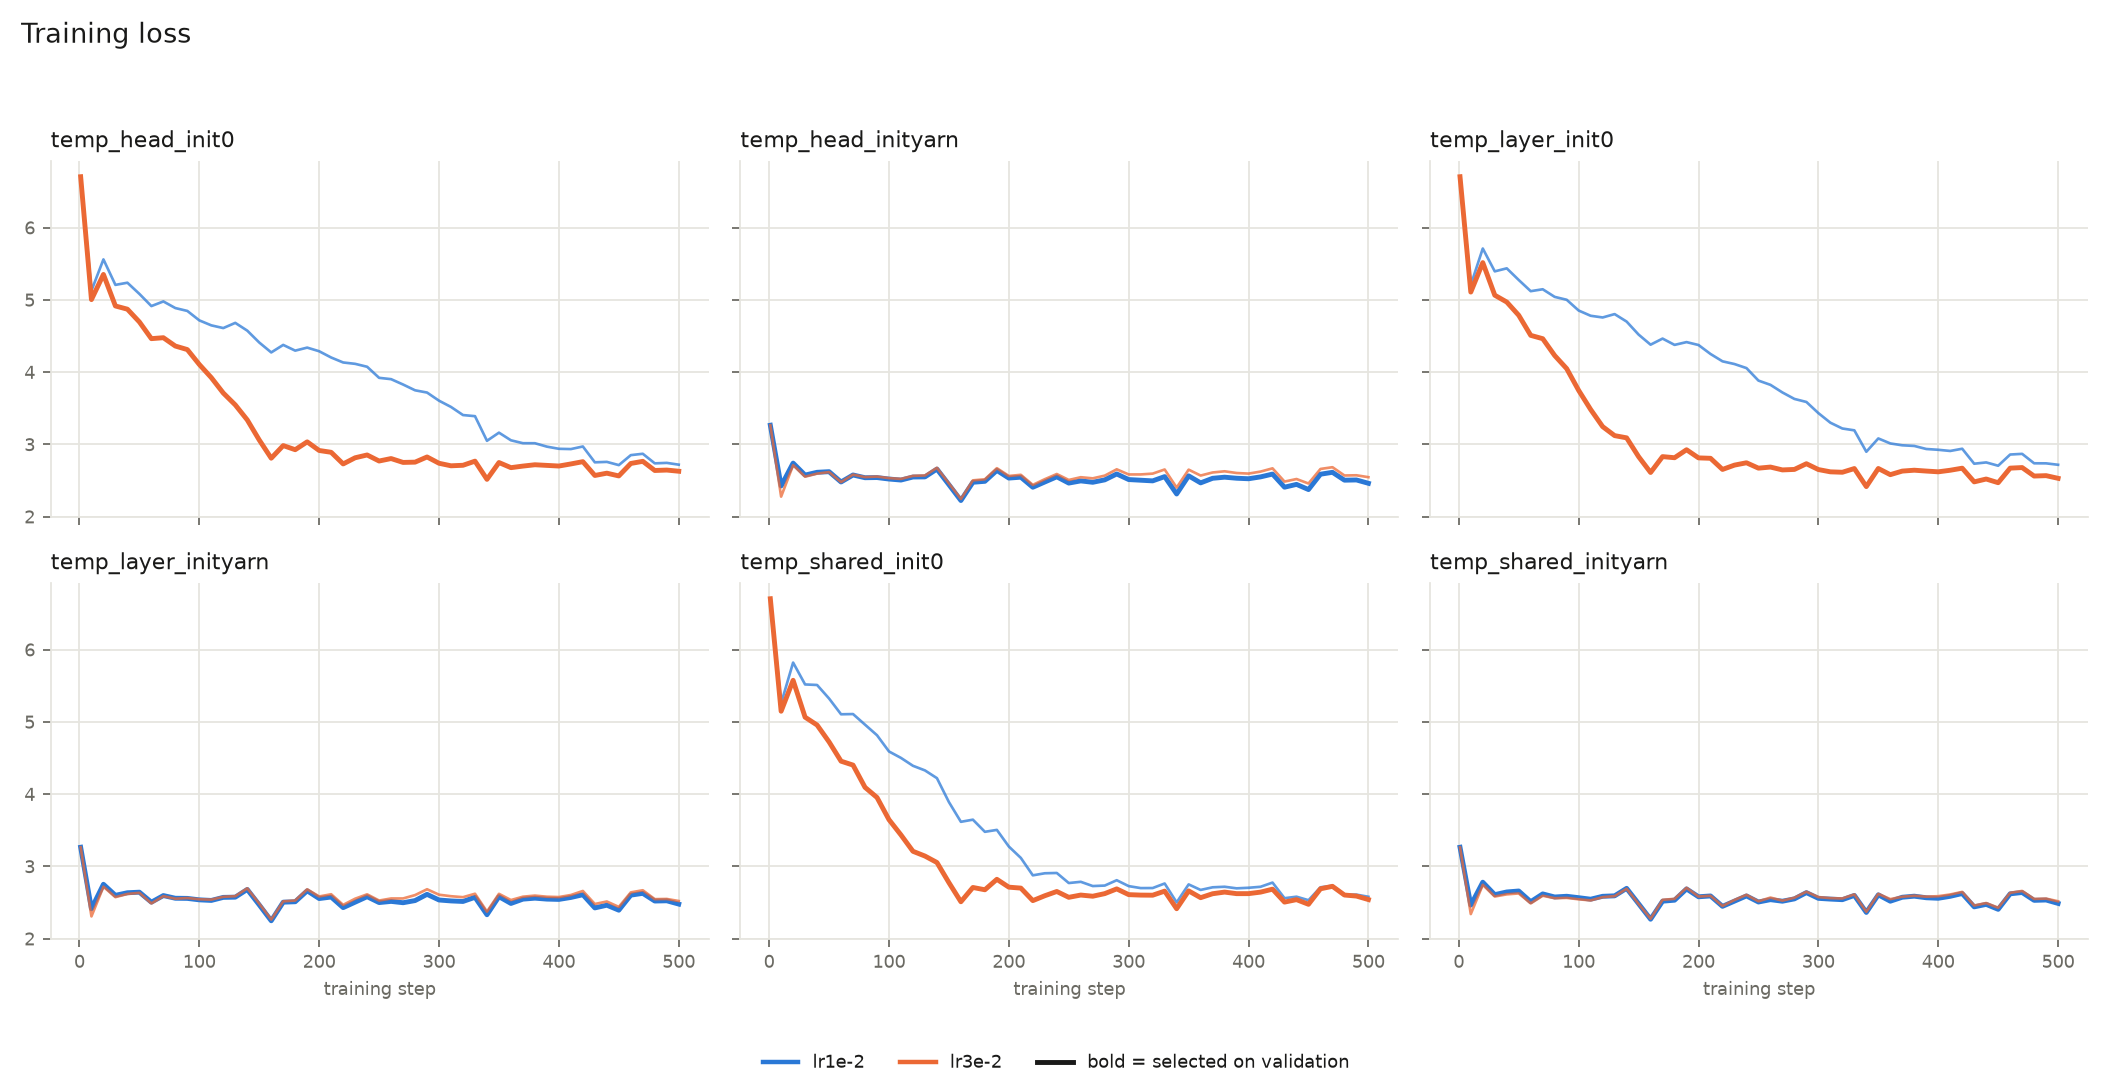
\includegraphics[width=\textwidth]{loss.png}
  \caption{Training loss of the frequencies + temperature runs for each
  granularity and starting point, at two learning rates (bold: chosen on
  validation). Runs started at YaRN begin near their final loss; runs from
  $a{=}0$ need hundreds of steps.}
  \label{fig:loss}
\end{figure*}

% Figure paths are set by \graphicspath in results.tex.

\begin{figure}[!h]
  \centering
  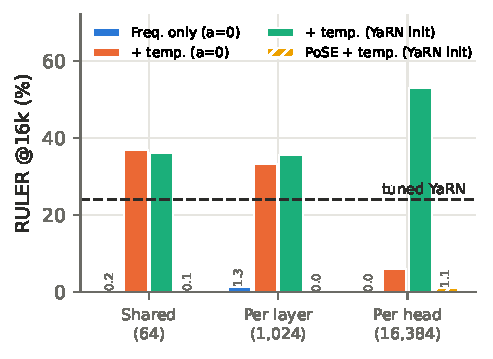
\includegraphics[width=\columnwidth]{fig_ablation_16k.pdf}
  \caption{RULER at 16k per granularity. Blue vs.\ orange differ only in the
  learned temperature; green starts both at YaRN; hatched yellow is PoSE
  (trained on 4k text). Dashed: tuned YaRN.}
  \label{fig:ablation}
\end{figure}

\begin{figure}[!h]
  \centering
  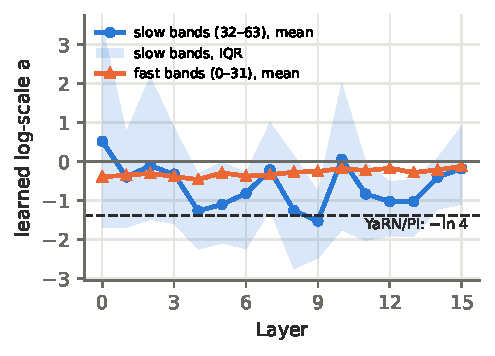
\includegraphics[width=\columnwidth]{fig_learned_a.pdf}
  \caption{Learned log frequency scales $a$ of the per-layer, frequencies-only
  model ($a<0$: slower rotation, $a=0$: unchanged). Line: mean over bands;
  shaded: middle 50\% of slow bands. Dashed: the single value YaRN and PI use
  for slow bands.}
  \label{fig:learned-a}
\end{figure}

\begin{figure}[!h]
  \centering
  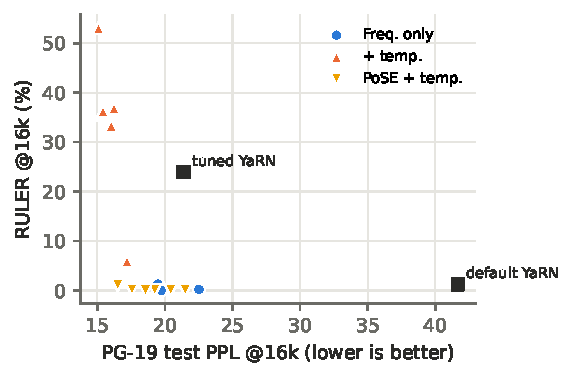
\includegraphics[width=\columnwidth]{fig_ppl_vs_ruler.pdf}
  \caption{Perplexity and retrieval at 16k disagree. Each marker is one trained
  model. Frequencies-only models (blue) and PoSE models (yellow) have perplexity
  similar to or better than tuned YaRN but almost no retrieval.
  The original model and PI are off the scale and not shown.}
  \label{fig:ppl-ruler}
\end{figure}

\begin{figure*}[!t]
  \centering
  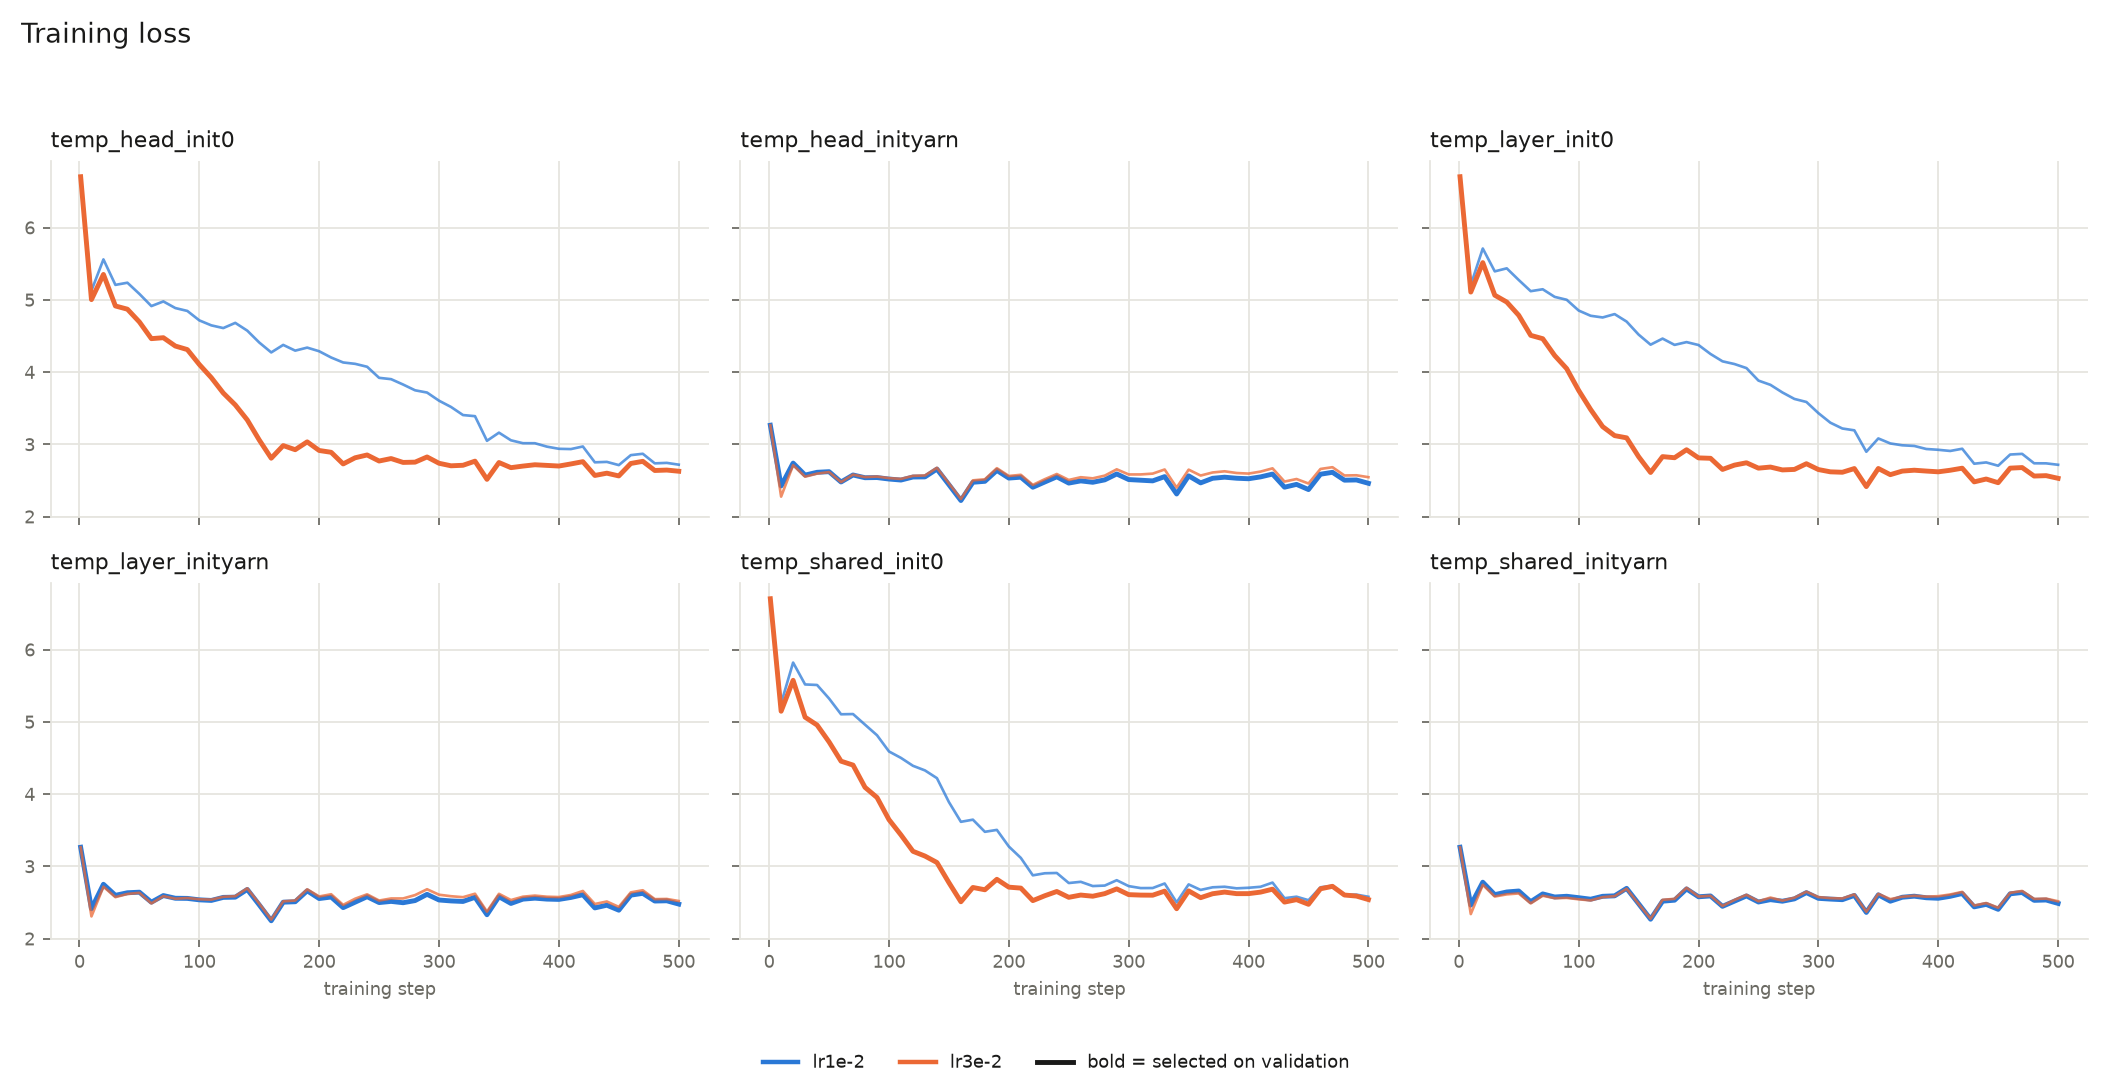
\includegraphics[width=\textwidth]{loss.png}
  \caption{Training loss of the frequencies + temperature runs for each
  granularity and starting point, at two learning rates (bold: chosen on
  validation). Runs started at YaRN begin near their final loss; runs from
  $a{=}0$ need hundreds of steps.}
  \label{fig:loss}
\end{figure*}
